% !TEX encoding = UTF-8 Unicode
% LaTeX file for resume 
% This file uses the resume document class (res.cls)

\documentclass{res} 
\usepackage{fontspec}
\usepackage{xeCJK}
\usepackage{listings}
\lstset{language=C,
numberstyle=\footnotesize,
basicstyle=\ttfamily\footnotesize,
numbers=left,
stepnumber=1,
frame=shadowbox,
breaklines=true}
\setCJKmainfont{STHeiti} % chinese type
%\setCJKmainfont{BiauKai}
%\usepackage{helvetica} % uses helvetica postscript font (download helvetica.sty)
%\usepackage{newcent}   % uses new century schoolbook postscript font 
\setlength{\textheight}{9.5in} % increase text height to fit on 1-page 
\usepackage{enumitem}

\XeTeXlinebreakskip = 0pt plus 1pt 

\begin{document} 


\name{\LARGE Real Time System Project1 Report}     % the \\[12pt] adds a blank
				        % line after name
\address{\\R03922106 蔡佑隆 unzledick@yahoo.com.tw\\ R04922067 楊翔雲 morris821028@gmail.com}

\begin{resume}

\section{\large 安裝 Linux Kernel 步驟解釋}
\begin{itemize}[leftmargin=-1.em]
	\item \lstinline{apt-get install fakeroot build-essential kernel-package libncurses5 libncurses5-dev}: 
	Ubuntu 安裝套件 \lstinline{fakeroot} 、 \lstinline{build-essential} 、 ... 等。
	\begin{itemize}
		\item \lstinline{fakeroot}: 模擬 root 權限執行指令,實際上並沒有 root 權限 (因遠端無法取得 root 權限)。
		\item \lstinline{build-essential}: 安裝 GNU Mach 需要 \lstinline{build-essential} package,包含 linux 開發的必要工具。
		\item \lstinline{libncurses libncurses5-dev}: 為 Linux 介面的圖形函數庫與開發工具。
	\end{itemize}
	\item \lstinline{sudo wget https://cdn.kernel.org/pub/linux/kernel/v2.6/lon gterm/v2.6.32/linux-2.6.32.68.tar.xz}: 從 Linux 官網下載 2.6.32.68 的 kernal 版本 (最新的版本為 4.x.x),用 root 權限安裝到 \lstinline{/usr/src} 中。
	\item \lstinline{make mrproper}: 刪除編譯過程中的目標檔案以及設定檔,連以前的 kernel 設定檔一起刪掉,原則上只有第一次執行核心編輯前才進行這個動作。
		\begin{itemize}
			\item \lstinline{make clean}: 不會刪除設定檔,僅編譯過程產生的中間檔案。
		\end{itemize}
	\item \lstinline{make menuconfig}: 在開機的圖形介面設定。重新啟動時,利用方向鍵選擇舊的 kernel 進行開機。
	\item \lstinline{make bzImage}: 編譯 kernel 且這個 kernel 是經過壓縮,步驟也很長。
	\item \lstinline{make module}: 將上一個步驟產出的模組,進行編譯,速度取決於 \lstinline{make bzImage}
	\item \lstinline{make modules_install}: 安裝 modules,如安裝版本 2.6.32.68,模組檔案會產生於 \lstinline{/lib/modules/2.6.32.68}。
	\item \lstinline{make install}: 安裝 \lstinline{bzImage} 建立好的模組。
	\item  \lstinline{#GRUB_HIDDEN_TIMEOUT=10, #GRUB_HIDDEN_TIMEOUT_QUIET=true}: 強迫顯示出 grub 選單,進入舊的 kernel 使用。
	\item \lstinline{update-grub2}: 將 grub 更改的內容更新至 grub.cfg (GBUB2 利用它來設定進入 BIOS)
\end{itemize}


\section{\large 遭遇問題}
\begin{itemize}[leftmargin=-1.em]

	\item 在Virtual Box上make menuconfig時解析度不夠,畫面放不下
		\begin{itemize}	
		\item[] Sol:使用Virtual Box的Insert Guest Additions CD image可以更改解析度
		\end{itemize}
	\item Thread create完thread 1比thread 0先run
	\begin{itemize}
		\item[] Sol:使用barrier在印出running前先做synchronization
	\end{itemize}
	\item 由於VM只有一個core,所以有沒有設cpu affinity並沒有影響執行結果
	\item 沒有用root權限無法正確FIFO
\end{itemize}


\section{\large Result}
\begin{figure}[htp]
    \begin{center}
        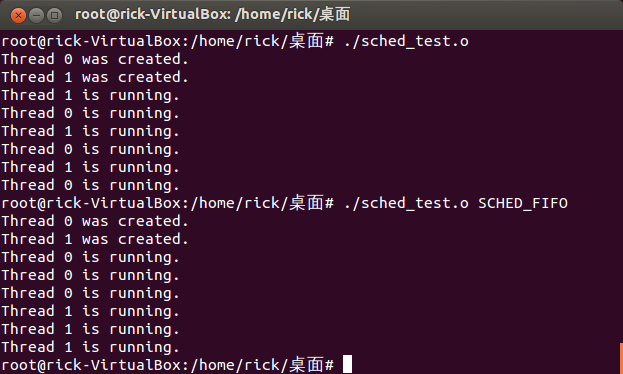
\includegraphics[width=300pt]{images/result.png}
        \caption{執行結果}
        \label{fig:result}
    \end{center}
\end{figure}
\end{resume}



\end{document}